% !TeX encoding = UTF-8
% !TeX program = xelatex
\documentclass[12pt, a4paper]{article}
\usepackage{xeCJK} % 须放在\usepackage{}列中足够前的位置
\usepackage{fontspec}
\usepackage{graphicx}
\usepackage{caption}
\usepackage{enumerate}
\usepackage{setspace}
\usepackage{array} % 製作表格必須的宏包
\usepackage{tabularx} % 自動調整列寬的表格宏包
\usepackage{adjustbox}
\usepackage{ulem} % 包含 ulem 宏包
\usepackage{amsmath}

\setCJKfamilyfont{heiti}{Heiti TC}
\CJKfamily{heiti}
\setmainfont{Arial}
\setstretch{1.5}


\begin{document}
\begin{center}
  {\Huge 邏輯設計實驗} \\[2.5cm]
  {\Huge Lab9} \\[1.5cm]
  {\Huge 組合應用電路} \\ [4.5cm]
  \hspace{.6in}
  \begin{minipage}[t]{.4\linewidth}
    {\Large 班級:資訊一甲}\\[0.5cm]
    {\Large 學號:D1109023}\\[0.5cm]
    {\Large 姓名:楊孟憲}
  \end{minipage}    
\end{center}

\newpage
%\fontsize{30pt}{36pt}\selectfont 
%\normalsize

\begin{description}
  \fontsize{22pt}{25pt}\selectfont 
    \item [一、]摘要 
      \begin{enumerate}
        \fontsize{20pt}{22pt}\selectfont
          \item 加法器 
            \begin{description}
              \fontsize{16pt}{20}\selectfont
                \item[(1)] 電路邏輯 \\
                  \begin{samepage}
                    \fontsize{14pt}{16pt}\selectfont
                    將兩個 4 bits 的二進位數字相加。 \\
                    $\bullet$ Cin 代表前一位的進位 \\
                    $\bullet$ Cout 代表最後的進位 \\
                  \end{samepage}
                \item [(2)] 7483\space IC \\[.4cm]
                  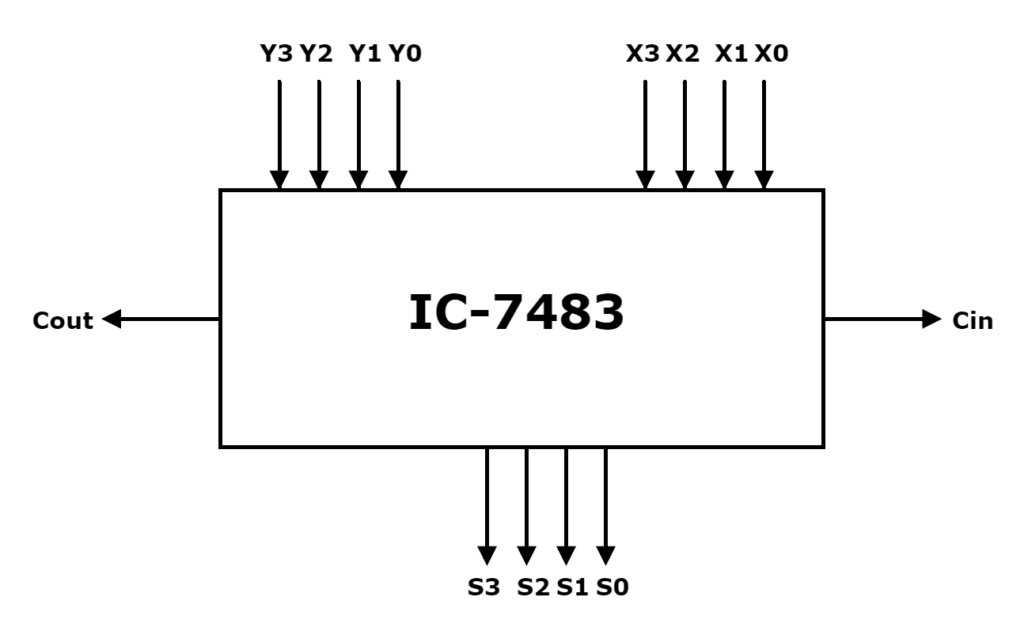
\includegraphics[width=10cm]{./image/addition.png} \\
              \normalsize
            \end{description}
            \item 2 $\rightarrow$ 1 多工器\\
              \fontsize{16pt}{20pt}\selectfont
              \begin{samepage}              
                三個輸入 A, B, S,S 代表選擇器。\\[.8cm]
              \end{samepage}
              \begin{description}
                  \item [(1)] 選擇碼真值表
                    \begin{table}[h]
                      \centering
                      \label{tab:sample}
                      \begin{adjustbox}{width=.15\textwidth}
                      \begin{tabular}{ |c|c| }
                        \hline
                        S & Y \\
                        \hline
                        0 & B \\
                        \hline
                        1 & A \\
                        \hline
                      \end{tabular}
                      \end{adjustbox}
                      \end{table} \\
                  \item [(2)] 組合函示表示式\\ 
                      $Y = A\cdot S + B\cdot \bar S$
                  \item [(3)] MUX IC \\
                      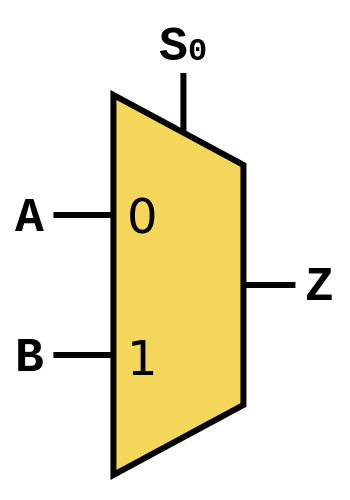
\includegraphics[width=5cm]{./image/Multiplexer_2-to-1.svg.png}
              \end{description}
              
              \fontsize{20}{22}\selectfont
              \item BCD加減法
                \begin{description}
                  \fontsize{16}{18}
                  \item[(1)] 加法 \\
                    \begin{samepage}
                      \fontsize{14}{16}\selectfont
                      將兩個 BCD 碼相加,先將兩兩相加,如果加起來超過 $(1001)_{bcd}$ 再將結果加上 $(0110)_{bcd}$。
                      \\例如:$(1000)_{bcd} + (0011)_{bcd}$ 出來的結果為 \sout{$(1011)_{bcd}$}, 因為超過 BCD 碼 $(1001)_{bcd}$
                      所以要再加上 $(0110)_{bcd}$ 並進位,正確答案為 $(10001)_{bcd}$
                    \end{samepage}
                  \fontsize{16}{18}\selectfont
                  \item[(2)] 減法 \\
                    \begin{samepage}
                      \fontsize{14}{16}\selectfont
                      先將負數做2的補數再做相加,如果加起來超過 $(1001)_{bcd}$ 再將結果加上 $(0110)_{bcd}$。
                    \end{samepage}
                \end{description}
        \normalsize
      \end{enumerate}
    \item [二、]實驗結果
      \begin{description}
        \fontsize{20pt}{22pt}\selectfont
        \item 實驗 (BCD 加法器)
          \fontsize{16pt}{18pt}\selectfont
            \begin{description}
              \item [$\bullet$] 設計一個BCD加法器, 輸入為兩個BCD數字, 輸出為其總和.
              \fontsize{18pt}{20pt}\selectfont
                \item [(1)]設計邏輯 \\[.3cm]
                \begin{samepage}
                  \fontsize{16pt}{18pt}
                    使用 7483 加法器,將兩數相加。\\
                    
                    \begin{description}
                      \bf
                      \item[$\bullet$] 如何判斷進位 \\
                        \begin{samepage}
                          \normalfont
                          已知 BCD 最大為 (1000),所以當 S4 = 1 時, S2、S3 不能等於 1,或者當二進位加法最後有進位,就代表需要進位,有了這個邏輯就可以幫助我們實作電路了。\\[.5cm]
                          判斷進位邏輯閘:\\
                          $c = (S4\cdot S3) + (S4\cdot S2) + Cout$
                        \end{samepage}

                      \item[$\bullet$] 進位處理 \\
                      \begin{samepage}
                        \normalfont
                        當兩數相加後的結果超過 (1001) 就需要將結果加上 (0110) 校正。
                        我們這時可以再利用 一顆 7483 加法器加上4 bits 的數字,已知這4 bits 的 B1 和 B4 都為零,所以可以直接接地。
                        B2, B3 可以接上進位判斷。
                      \end{samepage}                        
                    \end{description}
                  
                \end{samepage}
              
              \item [(2)] 電路圖 \\[.5cm]
                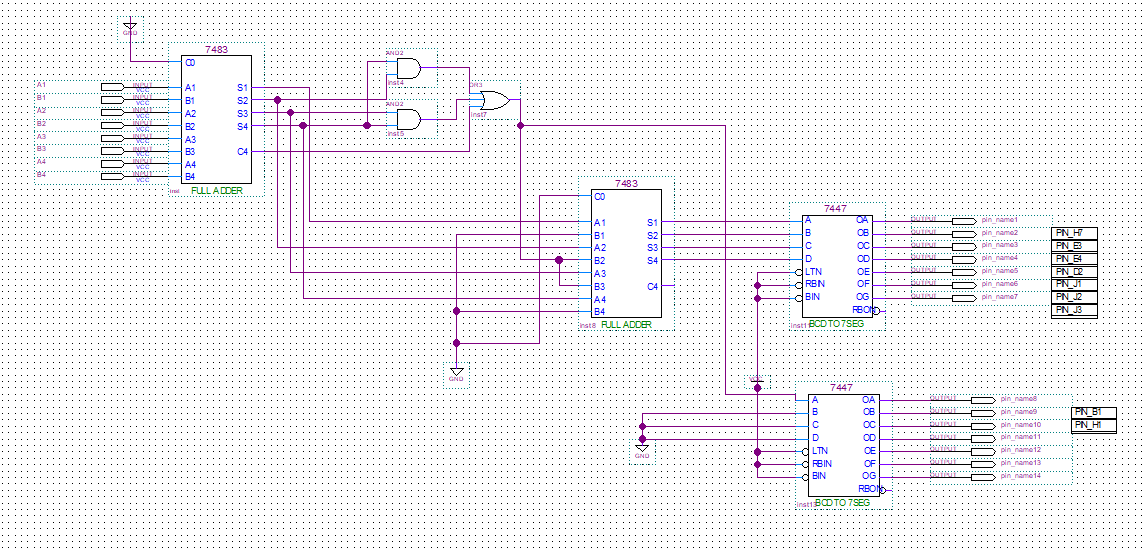
\includegraphics[width=13cm]{./image/ex1.png} \\
            \end{description}

        \fontsize{20}{22}\selectfont
        \item 實驗(有號數) \\[.3cm]
            \fontsize{16}{18}\selectfont
            $\bullet$ 設計一個組合電路,輸入為 4-bit binary 有號數 (2’complement 表示法)\\
            $\bullet$ 輸出此數字的絕對值 |A| 及對應的正負號 Sign 
            \begin{description}
              \item[(1)] 邏輯設計\\
                \begin{samepage}
                    假設是正數就直接輸出,否則輸出 2 的補數。
                    我們知道2的補數可以先做 1 的補數再加一。
                    而一的補數就是將1變0、0變1。\\
                    
                    我們可以利用 XOR 閘的特性同時完成判斷以及補數,任何值 XOR 1 等於該反向、XOR 0 等於自己
                    。將 input 的前 3 bit XOR sign bit。即可完成判斷及做1的補數,此時如果要做補數的話要再加一,因為前面XOR 是做 1 的補數。
                    這時候我們再利用 7483 來加 1,而代表一的那個 bit 就是 sign bit,如此一來,當輸入為負數就會做一的補數再加一,否則不做補數再加零。
                    $$ f_{boolen}=\left\{
                      \begin{aligned}
                      S_1 & = & A_1 \oplus A_4 + A_4 \\
                      S_2 & = & A_2 \oplus A_4 + A_4 + Carry \\
                      S_3 & = & A_3 \oplus A_4 + A_4 + Carry\\
                      S_4 & = & Carry \\
                      Sign bit & = & A_4
                      \end{aligned}
                      \right.
                      $$
                      
                  \end{samepage}
              \item[(2)] 電路圖\\[.3cm]
                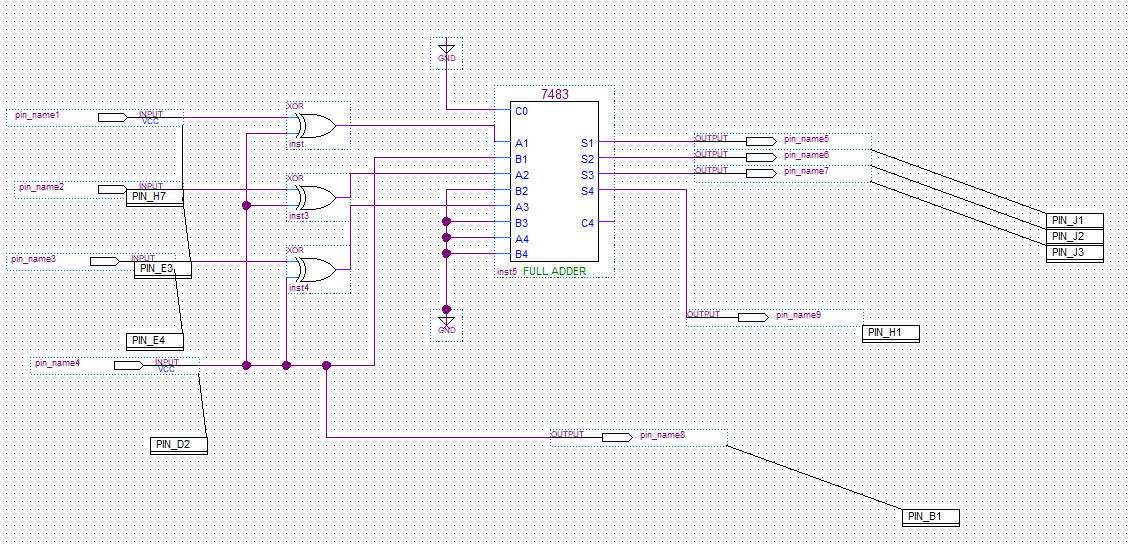
\includegraphics[width=13cm]{./image/ex2.png} 
            \end{description}
        \normalsize    
      \end{description}


    \item [三、]問題討論心得 \\[.6cm]
      \begin{minipage}[t]{\linewidth}
        \fontsize{16}{18}\selectfont
          這次實驗為組合電路,從頭到尾設計一套邏輯,利用之前課程所學的邏輯閘,設計電路並完成實驗題目所需。
          本次實驗第二題大部分的人使用 MUX 多工器來實作。我觀察到XOR邏輯閘可以同時解決補數以及判斷正負號,設計了一套絕對值電路。也成功用更精簡的方法做出此題。
        \normalsize  
      \end{minipage}
  \normalsize
\end{description}

\end{document}

